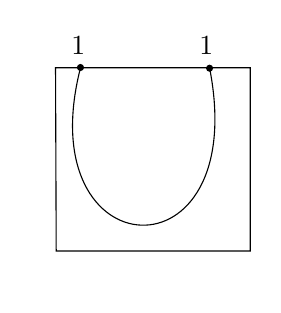
\begin{tikzpicture}[yscale=-1,scale=0.015,baseline={([yshift=-.5ex]current bounding box.center)}]
\begin{scope}[shift={(0.00mm,719.29mm)}]
% path id='path3338'
% path spec='m 34.267833,-564.76366 1648.607167,0 0,1551.42947 -1642.892757,0 z'
\draw [fill=none,draw=black] (34.27mm,-564.76mm)
-- ++(1648.61mm,0.00mm)
-- ++(0.00mm,1551.43mm)
-- ++(-1642.89mm,0.00mm)
-- cycle
;
% path id='path3342'
% path spec='m 245.701,-564.44137 c -442.58878,1723.38657 1450.6354,1830.02727 1092.8091,0.18879'
\draw [fill=none,draw=black] (245.70mm,-564.44mm)
.. controls ++(-442.59mm,1723.39mm) and ++(357.83mm,1829.84mm) .. ++(1092.81mm,0.19mm)
;
\draw [fill=black,draw=black] (245.47mm,-566.91mm) circle (25mm) ;
\draw [fill=black,draw=black] (1338.45mm,-560.85mm) circle (25mm) ;
\node [black] at (226.27mm,-750.41mm) { $1$ };
\node [black] at (1311.18mm,-750.33mm) { $1$ };
\end{scope}
\end{tikzpicture}
